 \begin{center}
 \textbf{\dots\og vivre l’unité comme offrande de soi dans notre communauté \fg \dots}
 \end{center}
L’Église, fruit de l’attente du Père, du Fils, et de l’Esprit Saint travaille pour qu’advienne effectivement le Règne du Dieu Trine, règne de justice, de vérité et de paix.
En ce sens, elle attend qu’éclatent les bourgeons des cieux nouveaux et d’une nouvelle terre. Dieu offre au monde, à ses enfants que nous sommes, son Fils comme présent suprême. En nous l’offrant, Dieu nous indique la nature de ce qu’il faut offrir et la bonne manière de l’offrir. C’est ce qui coute, ce qui est cher, ce qui intègre le sacrifice qu’on offre et cette offrande se fait de manière pleine et totale en vue du bonheur de celui à qui est ordonné ce don.
C’est dans cette perspective que nous devrons vivre l’unité comme offrande de soi dans notre communauté de paroisses. En effet, l’unité, comme ce qui est appelé à former un tout, une jonction de plusieurs choses diverses les unes avec les autres, en vue de former un ensemble indivisible à l’intérieur duquel il y a communication, exige sacrifice et accueil de l’autre. Cette unité des fidèles doit renfermer, en son sein, les vertus de la tolérance, de la responsabilité, du pardon à donner net à recevoir, du respect d’autrui, de sa vie privée, de ses biens et de la vie en général.

En Dieu donc toutes choses sont une. En nous offrant le Fils qui est la pleine présence de la divinité, Dieu offre l’essence de l’unité à l’humanité.
\begin{wrapfigure}{l}{1.3cm}
\vspace{-0.5cm}
	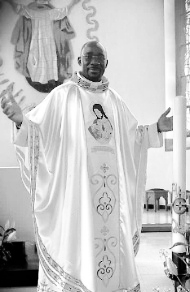
\includegraphics{../images/standing_daniel.png}
\end{wrapfigure}
Le Christ avant de quitter ce monde a formulé cette prière \textbf{\og Que tous soient UN\fg (Jn 17, 21)} cette demande au Père révèle toujours à ses enfants que nous sommes son identité unitaire.
Cela montre que nous sommes tous conduits par un même Esprit Saint pour former un seul corps qui vit dans l’espérance de la gloire à venir. Ainsi en sera-t-il de la vie en communauté. Notre unité devrait être de la réciprocité indicible du Père et de Jésus, modèle inaccessible. 

\begin{flushright}
Bonne méditation !
\textit{Père  Daniel  ETTÉ}
\end{flushright}


